% ОБЯЗАТЕЛЬНО ИМЕННО ТАКОЙ documentclass!
% (Основной кегль = 14pt, поэтому необходим extsizes)
% Формат, разумеется, А4
% article потому что стандарт не подразумевает разделов
% Глава = section, Параграф = subsection
% (понятия "глава" и "параграф" из стандарта)
\documentclass[a4paper,article,14pt]{extarticle}

% Подключаем главный пакет со всем необходимым
\usepackage{spbudiploma}

% Пакеты по желанию (самые распространенные)
% Хитрые мат. символы
\usepackage{euscript}
% Таблицы
\usepackage{longtable}
\usepackage{makecell}
% Картинки (можно встявлять даже pdf)
\usepackage[pdftex]{graphicx}

\usepackage{amsthm,amssymb, amsmath}
\usepackage{textcomp}

\usepackage{mathtools}
\DeclarePairedDelimiter\ceil{\lceil}{\rceil}


\begin{document}

% Титульник в файле titlepage.tex
% --------------------- Стандарт СПбГУ для ВКР --------------------------
% Автор: Тоскин Николай, itonik@me.com
% Если заметили ошибку, напишите на email
% Если хотите добавить изменение самостоятельно, GitHub: . PR-s welcome!
% Использованы материалы:
% habr.com/ru/post/144648/
% cpsconf.ru
% Текст:
% http://edu.spbu.ru/images/data/normativ_acts/local/20181030_10432_1.pdf
% Титульный лист:
% http://edu.spbu.ru/images/data/normativ_acts/local/20180703_6616_1.pdf
% -----------------------------------------------------------------------

% Титульный лист диплома СПбГУ
% Временное удаление foot на titlepage
\newgeometry{left=30mm, top=20mm, right=15mm, bottom=20mm, nohead, nofoot}
\begin{titlepage}
\begin{center}
% Первый символ съедается, первым знаком поставлен Ы
\textbf{Санкт--Петербургский}
\textbf{государственный университет}

\vspace{35mm}

\textbf{\textit{\large Романычев Леонид Романович}} \\[8mm]
% Название
\textbf{\large Выпускная квалификационная работа}\\[3mm]
\textbf{\textit{\large Апостериорный анализ и оценка эффективности алгоритмов}}

\vspace{20mm}
% Булшит
Уровень образования: бакалавриат\\
Направление 02.03.02 «Фундаментальные информатика и информационные технологии»\\
Основная образовательная программа СВ.5003.2017
«Программирование и информационные технологии»\\
Профиль «Автоматизация научных исследований»\\[30mm]


% Научный руководитель, рецензент
% Сходить в уч отдел и узнать, правильно ли
\begin{flushright}
{Научный руководитель:} \\
к. ф.-м. н. доцент кафедры моделирования\\
электромеханических и компьютерных систем,\\
Никифоров Константин Аркадьевич
\end{flushright}
\begin{flushright}
{Рецензент:} \\
к. ф.-м. н. доцент кафедры радиофизики и электронных систем\\
Северо-Восточного федерального университета им. М.К. Аммосова»,\\
Антонов Степан Романович
\end{flushright}

\vfill 

{Санкт-Петербург}
\par{\the\year{} г.}
\end{center}
\end{titlepage}
% Возвращаем настройки geometry обратно (то, что объявлено в преамбуле)
\restoregeometry
% Добавляем 1 к счетчику страниц ПОСЛЕ titlepage, чтобы исключить 
% влияние titlepage environment
\addtocounter{page}{1}


% Содержание
\tableofcontents
\pagebreak

\specialsection{Введение}

Алгоритмы являются одной из важнейших составляющих эффективной программной системы. В больших проектах правильно написанный алгоритм может сэкономить компании миллионы долларов. Например, в 2016 году социальная сеть ``ВКонтакте'', оптимизировав работу с личными сообщениями, сэкономила минимум 5 млн. долларов [1].

В разработке таких алгоритмов не обойтись без предварительного анализа: нужно уметь оценивать те или иные ресурсы, которые алгоритм потребляет во время работы. Самый распространенный ресурс --- это время выполнения алгоритма. Он является важнейшим, так как пользователи не любят ждать. Второй по значимости ресурс --- это память. Причем, если время выполнения алгоритма вычисляется как количество базовых операций и связано с функцией трудоемкости алгоритма, то память обычно берется не как суммарное количество памяти, которое потребляет алгоритм, а как количество дополнительной памяти, при этом память связана с функцией объема памяти алгоритма.

Обычный асимптотический анализ не всегда точен для конечного диапазона длин входов из-за часто больших коэффициентов у компонентов функций ресурсной эффективности:
$$\Psi_A(D) = C_V \cdot V_A(D) + C_f \cdot f_A(D),$$
где $V$ --- объем потребляемой алгоритмом $A$ памяти, $f$ --- трудоемкость.

В данной работе будет рассмотрен новый подход на основе эмпирического анализа: по данным, полученным экспериментальным путем, будет построена функция доверительной ресурсоемкости (доверительной памяти) с выбранным коэффициентом доверия, а также для упрощения процесса разработана автоматизированная система в виде сайта.

\pagebreak

\specialsection{Постановка задачи}

Для вычисления доверительной ресурсоемкости необходимы данные, полученные многократным запуском программных реализаций исследуемых алгоритмов. После проведения большого числа экспериментов строится доверительный интервал оцениваемой величины ресурсоемкости с заданной доверительной вероятностью.

Данная работа включает в себя следующие этапы:
\begin{enumerate}
\item Выбор подходящего для демонстрации алгоритма.
\item Реализация этого алгоритма и многократный запуск для получения данных.
\item Этап предварительного исследования. Этап необходим для проверки нулевой гипотезы о законе распределения данных.
\item Этап основного исследования.
\item Построение автоматизированной системы для проведения вышеописанного анализа.
\end{enumerate}


\pagebreak

\specialsection{Обзор литературы}

В 1936 году Алан Тьюринг предложил модель формализации понятия алгоритма с помощью машины Тьюринга. На базе этой модели в работах [2, 3] были сформулированы первые подходы для оценки алгоритмов:
\begin{itemize}
\item оценка сложности программной реализации алгоритма;
\item оценка сложности вычислительного процесса, задаваемого алгоритмом.
\end{itemize}

В первом подходе оценку сложности связывают с качеством информации, которая содержится в записи алгоритма [4] или с объемом программной реализации алгоритма.
Во втором подходе для оценки сложности вычислительного процесса необходимо вводить меру сложности вычислений, задаваемых алгоритмом для решения конкретных задач. 

В зависимости от того, когда производится анализ (до или после реализации алгоритма), его можно разделить на два этапа:
\begin{enumerate}
\item Априорный (или теоретический) анализ — анализ алгоритма перед
его запуском на электронно-вычислительной машине.
\item Апостериорный (или экспериментальный) анализ — анализ алгоритма выполняется только после его запуска на электронно-вычислитель-
ной машине с определенными комплектующими.
\end{enumerate}

Априорный анализ использует только асимптотические оценки сложности алгоритма, зависящие от входных данных и их размеров. Методы априорного анализа хорошо представлены в работах [5, 6, 7].

Новый подход к анализу был предложен в работе [8] для повышения точности результатов эмпирического анализа алгоритма. Авторы фиксируют размер входных данных, проводят эксперименты и на основе собранных данных строят доверительный интервал функции трудоемкости алгоритма с заданным коэффициентом доверия. Для аппроксимации значений трудоемкости используется бета-распределение. Такой подход на практике показывает более реальные границы сложности алгоритма.

Описанный метод включает в себя два этапа:
\begin{enumerate}
\item предварительный этап — проверка гипотезы о законе распределения
трудоемкости алгоритма как ограниченной дискретной случайной величины [9];
\item основной этап — определение значения доверительной трудоемкости $f_{\gamma}(n)$ в зависимости от длины $n$ исследуемого алгоритма [8].
\end{enumerate}

\begin{figure}[h!]
\center{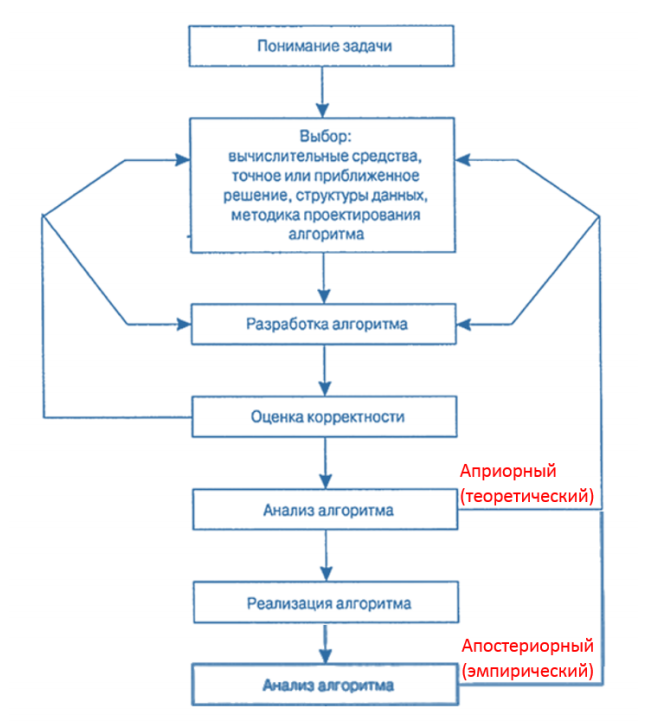
\includegraphics[width=0.7\linewidth]{images/scheme.png}}
\caption{Схема этапов при разработке алгоритма}
\label{ris:image1}
\end{figure}

За последние 10-15 лет машинное обучение вошло во множество научных и прикладных сфер. В частности методы машинного обучения были предложены для анализа сложности алгоритмов [10]. Можно ожидать, что в будущем эти методы будут дополняться и улучшаться.

Также стоит отметить, что в эпоху таких энергозатратных технологий как blockchain исследовать алгоритмы в апостериорном анализе можно не только на трудоемкость и ресурсоемкость, но также и на энергоэффективность [11]. В данный момент литературы по данной теме крайне мало.

\pagebreak

\section{Исследование ресурсоемкости}
\subsection{Общие положения исследования}

Основной целью исследования является построение доверительной
функции ресурсоемкости для рассматриваемого алгоритма. В дальнейшем будем использовать следующее общепринятое определение функции объема памяти (ресурсоемкости) [12, 13]:
\par
\textbf{Определение.} Функция объёма памяти. Под объёмом памяти, требуемым алгоритмом $A$ для входа, заданного множеством $D$, будем понимать максимальное число ячеек памяти информационного носителя модели вычислений, задействованных в ходе выполнения алгоритма.

Функцию объёма памяти алгоритма для входа $D$ будем обозначать через $V_A(D)$. Предполагается, что закон распределения значений $V_A(D)$ неизвестен.

Экспериментально исследование можно разделить на следующие этапы:
\begin{enumerate}
\item Вводится ограниченная дискретная случайная величина с неизвестным распределением.
\item На основе данных, полученных после многократного запуска алгоритма, строится гистограмма относительных частот.
\item Полученная гистограмма аппроксимируется некоторой функцией плотности распределения вероятностей.
\item Для доказательства корректности выбранной функции плотности распределения формулируется и доказывается гипотеза о распределении относительных частот значений функции ресурсоемкости. Если доказать гипотезу не удалось, необходимо выбрать другую функцию и повторить данный шаг.
\item После того, как гипотезу удалось доказать, для функции нужно выбрать коэффициент доверия $\gamma$.
\item Далее решается интегральное уравнение и находится значение $V_{\gamma}(n)$ ресурсоемкости.
\end{enumerate}

Найденное на последнем шаге значение и есть доверительная ресурсоемкость алгоритма. Его можно интерпретировать так: для единичного входа алгоритма, его ресурсоемкость будет заключена в сегмент $[V^{\vee}, V_{\gamma}]$, т. е. между лучшим случаем и значением $V_{\gamma}(n)$ с вероятностью $\gamma$.

\subsection{Построение гистограммы частот}

Перед построение гистограммы относительных частот необходимо нормировать данные. Введем случайную нормированную величину $T$. Ее реализации $t_i$ получаются на основе теоретических и эмпирических значений ресурсоемкости [8]:
$$t_i = \frac{V_i - V^{\vee}}{V^{\wedge} - V^{\vee}}$$
где $V_i$ — значение функции ресурсоемкости для сгенерированных случайных допустимых входов $D_i$: $V_i = V_A(D_i)$, $i = \overline{1, m}$, а $V^{\wedge}, V^{\vee}$ — теоретический максимум и минимум функции объема памяти соответственно. При этом отметим, что
нормированные величины $t_i$ принимают значения из сегмента [0, 1].

Далее необходимо определить количество полусегментов для построения гистограммы относительных частот. Существует множество способов это сделать. Воспользуемся эмпирическим правилом:
$$k = [\sqrt{n}],$$
где $n$ — общее число наблюдений.

\subsection{Определение объема выборки}

Для построения гистограммы относительных частот нужно определить размер выборки. Заметим, что не всегда имеется возможность проводить повторные эксперименты и исследователи вынуждены работать с уже полученными данными. Такое ограничение может быть связано с несколькими факторами, например, дороговизной или трудоемкостью. Но даже когда возможность проводить эксперименты есть, имеет смысл минимизировать размер выборки для сокращения дополнительных расходов. Возникает проблема определения минимального числа экспериментов $m$ для вычисления ресурсоемкости алгоритма при заданной доверительной вероятности $\gamma$. Заметим, что длина входа $n$ при этом остается постоянной.

\subsubsection{Метод с использованием схемы Бернулли}
При известной вероятности $p$ значений трудоемкости с наименьшей
частотной встречаемостью можно применить метод на основе схемы Бернулли [12]. Его суть заключается в том, что величина $p$ трактуется как
вероятность успеха и рассматривается событие $A$ — наблюдение как минимум одного успеха в $m$ испытаниях с заданной вероятностью $\gamma$. Сама
задача сводится к определению числа испытаний $n$ в схеме Бернулли:

$$P(A) = 1 - (1 - p)^m \geq \gamma,$$
\noindentоткуда можно получить требуемый объем выборки:

$$m \geq \ceil*{ \frac{ln(1 - p)}{ln(1 - \gamma)}}$$

\subsubsection{Метод на основе закона распределения}

Более общий метод основан на рассмотрении гипотезы о законе распределения функции трудоемкости алгоритма [9]. Поскольку закон распределения значений $V_A(D)$ неизвестен, вводится гипотеза, что значения функции трудоемкости являются ограниченной дискретной случайной величиной, которая распределена по одному из хорошо известных законов распределения. Суть данного метода сводится к тому, что для определения минимального объема выборки $m$ проводится ряд последовательных экспериментов с постоянной длиной входа $n$. Значение $n$ задается исследователями, как и начальный объем выборки $m$.

На каждой итерации извлекаются выборки размера $m$ и вычисляются значения ресурсоемкости. Далее рассчитывается ряд статистических величин: выборочное среднее $\overline{V_{\epsilon}}(m)$ и выборочная исправленная дисперсия $S^2$ , которые являются оценками теоретической ресурсоемкости $\overline{V_A}$ и теоретической дисперсии ресурсоемкости $\sigma^2_A$ соответственно. Требуемый объем выборки рассчитывается по формуле:

$$m^* = m^*(\delta, \gamma) = min m : P(|\overline{V_{\epsilon}}(m) - \overline{V_A}|) \leq \delta) \leq \gamma,$$

\noindentт. е. минимальный объем выборки нужно выбирать таким образом, чтобы средние значения в выборке $\overline{V_{\epsilon}}$ позволяли построить доверительный интервал длиной $2\delta$, который покрывал бы неизвестное значение $\overline{V_A}$ с надежностью $\gamma$.
При этом условием останова для описанной последовательности итераций является выполнение неравенства:

$$m^*_{(i+1)} < m^*_{(i)},$$

\noindentгде $m^*_{(i)}$ — рассчитанный минимальный объем выборки на итерации $i$.

\pagebreak
\section{Проведение экспериментального исследования функции объема памяти}
\subsection{Описание выбранного алгоритма}

Проводить анализ на ресурсоемкость имеет смысл для алгоритмов с неконстантным использованием дополнительной памяти. Например, алгоритм сортировки, который работает <<на месте>>, не подойдет т. к. размер дополнительной памяти будет равен или очень близко равен 0 вне зависимости от входа алгоритма. Подойдут алгоритмы, использующие такие структуры данных как stack, deque, queue. Простейший пример такого алгоритма --- Обход в ширину, который использует очередь для обхода графа.

Для исследования был выбран алгоритм Левита [14]. Этот алгоритм находит кратчайшие пути от одной вершины до всех остальных на графах без петель. Стоит отметить, что алгоритм Левита работает даже на графах, где существуют ребра отрицательного веса, но при этом не должно существовать отрицательных циклов.

Входными данными для алгоритма является граф $G$, представленный в виде упорядоченной совокупности множеств вершин $V$ и ребер $E$:
$G = (V, E)$. Оценка размера входных данных производится по размеру
множеств вершин и ребер. Пусть $n$ — количество вершин в множестве $V$, $m$ — количество ребер в множестве $E$: $n = |V|$, $m = |E|$. В качестве размера дополнительной памяти будем брать максимальный размер дэка, который будет зафиксирован во время выполнения алгоритма.

\subsection{Генерация данных}

Нужно генерировать связные ориентированные графы с $n$ вершинами и $m$ ребрами. Количество ребер возьмем $m = 10n$. В общем случае $n$  и $m$ будут зависеть от поставленной задачи.

Для генерации связного графа с $m$ ребрами воспользуемся следующим алгоритмом:
\begin{enumerate}
\item Сначала построим дерево. Для этого соединим вершину $i$ с вершиной $(i + 1)$, для $i = \overline{1, n-1}$.
\item $m - n - 1$ раз соединим две случайные вершины.
\end{enumerate}

Этот алгоритм будем использовать как для предварительного, так и для основного исследования.

\subsection{Этап предварительного исследования}

Выдвигается гипотеза, что функция ресурсоемкости алгоритма Левита имеет бета-распределение. Основные шаги предварительного исследования:

\begin{enumerate}
\item Фиксация значения длины входа $n = 1000$ из сегмента длин в области применения алгоритма.

\item Определение необходимого числа экспериментов $m = 10000$ (объем выборки).

\item Проведение экспериментального исследования и получение значений
ресурсоемкости $V_i$ для сгенерированных случайных допустимых входов $D_i: V_i = V_A (D_i), i = \overline{1, m},$

где $D_i$ - случайный допустимый вход, $V_A$ - алгоритм Левита.

Значение ресурсоемкости берется как максимальный размер очереди за время выполнения всего алгоритма.

\item Получение теоретических функций ресурсоемкости алгоритма для лучшего и худшего случаев. Функции $V_{A}^{\vee}$ и $V_{A}^{\wedge}$ для алгоритма Левита имеют вид:

$$V_{A}^{\vee}(n) = 1$$
$$V_{A}^{\wedge}(n) = n$$

Худший случай обоснован тем, что в любой момент времени в очереди находится не больше 1 вершины $v_i$. Вершин всего $n$, следовательно в очереди может находиться не более $n$ элементов.

\item Выбор числа $k = 100$ полусегментов для гистограммы относительных частот значений ресурсоемкости.

Значение $k$ получено через эмпирическое правило $$k = \sqrt{m}$$

\item Вычисление нормированного выборочного среднего и нормированной
исправленной выборочной дисперсии по формулам [9]:

$$\overline{t} = \frac{\overline{V_{t}}(n)- V^{\vee}}{V^{\wedge} - V^{\vee}}$$

$$s^2 = \frac{1}{m - 1} \sum\limits_{i=1}^m \frac{(V_i - \overline{V_t}(n))^2}{(V^{\wedge} - V^{\vee})^2}$$

где $V^{\wedge}$ и $V^{\vee}$ — соответственно максимальное и минимальное значение теоретических функций ресурсоемкости, $\overline{V_{t}}(n)$ — выборочное среднее.

\item Формулировка гипотезы об аппроксимирующем законе распределения и расчет параметров этого закона. В рассматриваемом случае
выдвигается гипотеза о бета-распределении.

Напомним, что случайная величина $X$ имеет бета-распределение, если она задаётся плотностью вероятности $V_X$, имеющей вид:

$$V_X(x) = \frac{1}{B(\alpha, \beta)}x^{\alpha - 1}(1 - x)^{\beta - 1},$$
где
 \begin{itemize}
\item $\alpha, \beta > 0$ произвольные фиксированные параметры, и
\item $B(\alpha, \beta) = \int_{0}^{1}x^{\alpha - 1}(1 - x)^{\beta - 1}dx$ — бета-функция.
\end{itemize}

Параметры бета-распределения рассчитываются по формулам [9]:

$$\alpha = \frac{\overline{t}}{s^2} (\overline{t} - (\overline{t})^2 - s^2)$$

$$\beta = \frac{(1 - \overline{t}}{s^2} (\overline{t} - (\overline{t})^2 - s^2)$$

В данном случае $\alpha = 2817, \beta = 677$.

\item Расчет теоретических частот по формуле функции плотности [9]:

$$p_i = \int_{x_i}^{x_i + \Delta x_i}  b(x, \alpha, \beta) dx,$$

где $b$ — функция бета-распределения.

\item Расчет наблюдаемого значения критерия согласия Пирсона по формуле [15]:

$$\chi ^2_{\text{набл}} = m \sum\limits_{i=1}^s \frac{(w_i - p_i)^2}{p_i},$$

где $w_i$ — относительные частоты.

\item Проверка гипотезы о законе распределения: если нулевая гипотеза
принимается, то осуществляется переход к основному этапу исследования. Иначе —
выбор другого закона распределения и повтор шагов 8–11.

В данном случае $\chi^2_{\text{набл}} = 109$, а $\chi^2_{\text{кр}} = 124$ (вычислено стандартной функцией пакета Microsoft Excel). Так как $\chi^2_{\text{набл}} < \chi^2_{\text{кр}}$, то нулевая гипотеза принимается.

\end{enumerate}

На рисунке 2 представлена гистограмма относительных частот, а так же аппроксимирующая ее функция.

\begin{figure}[h!]
\center{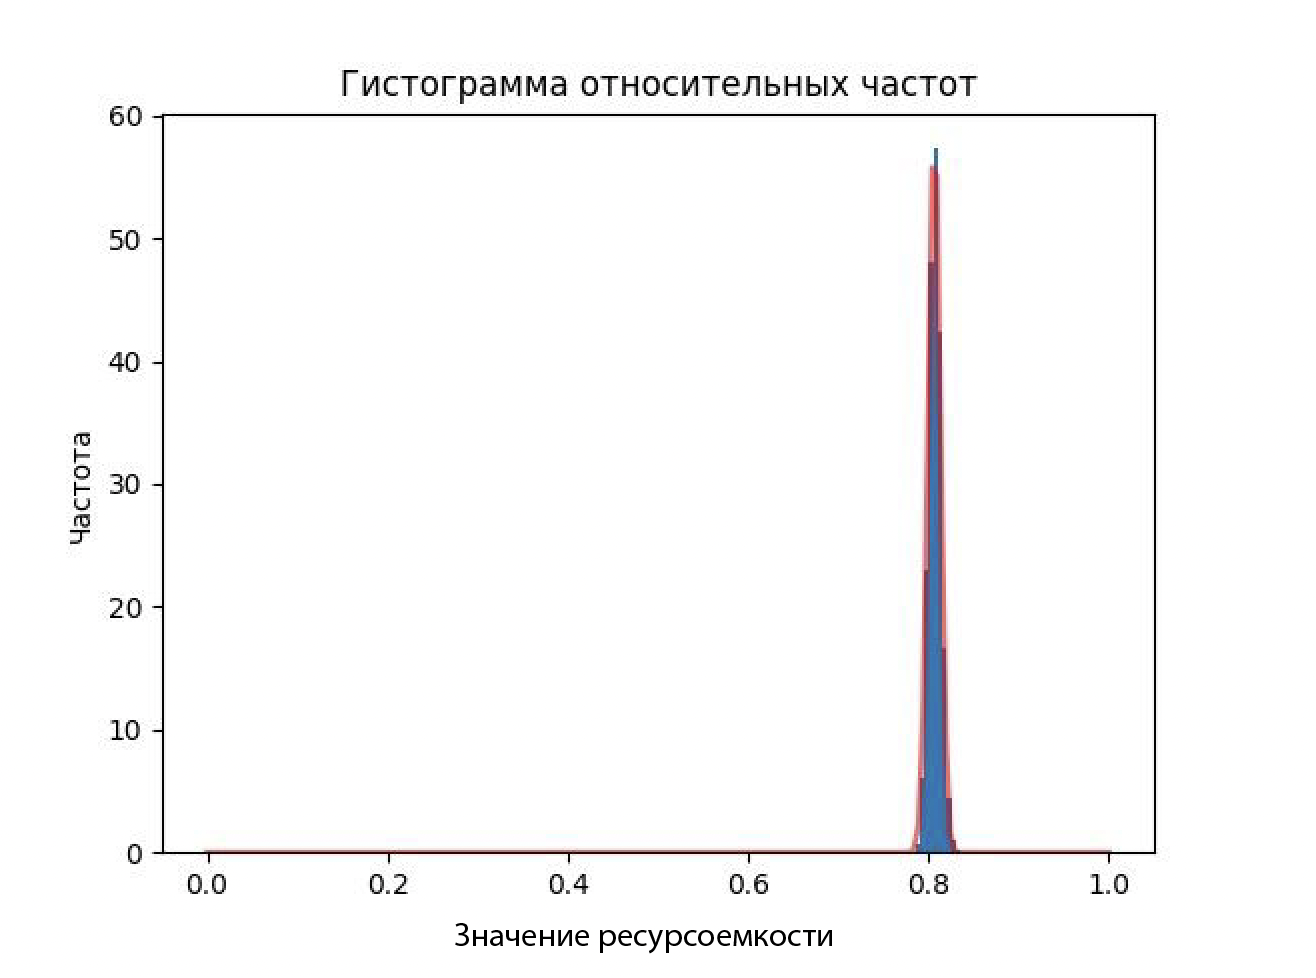
\includegraphics[width=0.7\linewidth]{images/gist.png}}
\caption{Теоретические и эмпирические частоты для алгоритма Левита при $n = 1000$ с разбиением нормированного сегмента $[0, 1]$ на 100 полусегментов}
\label{ris:image1}
\end{figure}

\subsection{Этап основного исследования}

Задача этапа основного исследования — построение функции доверительной ресурсоемкости на основе данных, полученных из экспериментального исследования.

\begin{enumerate}
\item Определение сегмента значений длин входа. В рассматриваемом случае алгоритма Левита будет применяться для графов с количеством вершин от 100 до 1400;

\item Выбор шага изменения длины входа для сегмента. Данный
шаг будет использоваться для проведения экспериментального исследования. В рассматриваемом случае значение шага равно 100;

\item Определение необходимого числа $m$ экспериментов с программной
реализацией алгоритма для фиксированной длины входа. В данном случае $m = 10000$. По итогам экспериментального исследования определяется выборочная средняя и дисперсия. 

\item Расчет на основе данных, полученных из экспериментального исследования, выборочной средней и дисперсии для каждого значения $n$.

\item Расчет на основе результатов, полученных на шаге 4, параметров
аппроксимирующего бета-распределения по формулам из прошлого раздела как
функций длины входа $\alpha(n)$, $\beta(n)$;

\item Определение значения коэффициента доверия и вычисление значений левого $\gamma$-квантиля бета-распределения [12]:

$$\delta_{I, Q}(\gamma) = B^{-1}(\frac{1}{2} + \frac{\gamma}{2}, \alpha, \beta) - B^{-1}(\frac{1}{2} - \frac{\gamma}{2}, \alpha, \beta)$$

\item Вычисление значений функции доверительной ресурсоемкости для исследуемого сегмента длин входа по формуле [8]:

$$V_{\gamma}(n) = V^{\vee}(n) + x_{\gamma}(n)(V^{\wedge} - V^{\vee})$$

\end{enumerate}


\begin{figure}[h!]
\center{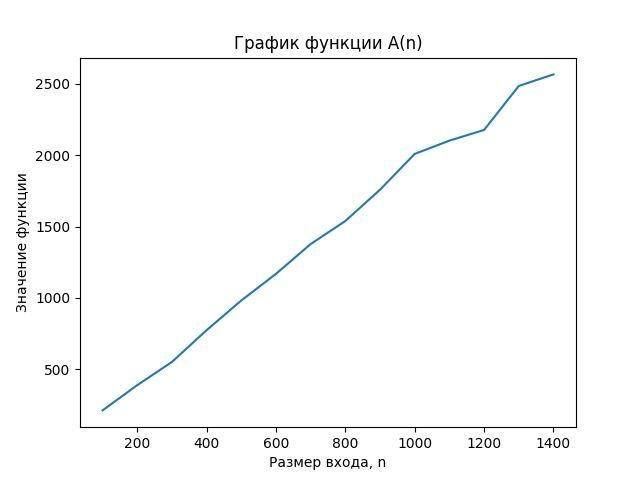
\includegraphics[width=0.7\linewidth]{images/2.jpeg}}
\caption{График функции $\alpha(n)$ — параметра $\alpha$ аппроксимирующего бета-распределения для алгоритма Левита}
\label{ris:image1}
\end{figure}

\begin{figure}[h!]
\center{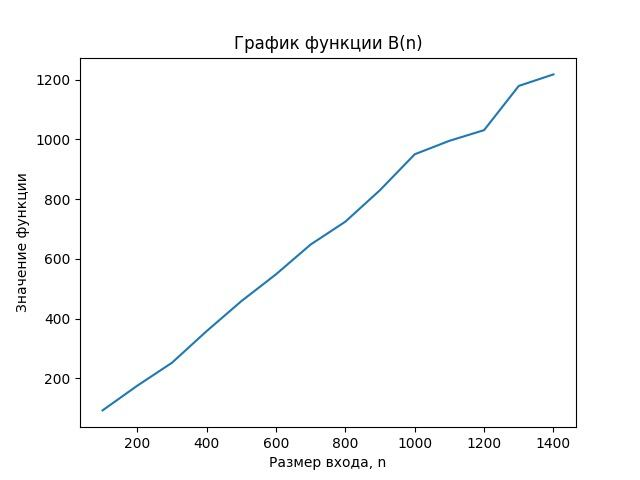
\includegraphics[width=0.7\linewidth]{images/3.jpeg}}
\caption{График функции $\beta(n)$ — параметра $\beta$ аппроксимирующего бета-распределения для алгоритма Левита}
\label{ris:image1}
\end{figure}
\newpage
\begin{figure}[h!]
\center{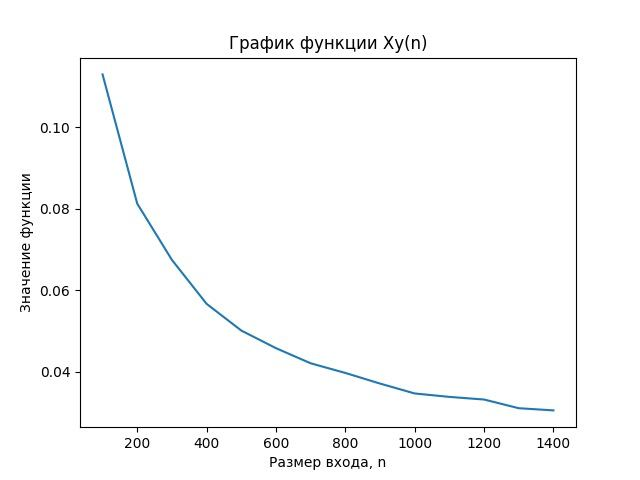
\includegraphics[width=0.7\linewidth]{images/4.jpeg}}
\caption{График зависимости левого $\gamma$-квантиля бета-распределения $x_{\gamma}(n)$ от длины входа для алгоритма Левита}
\label{ris:image1}
\end{figure}

\begin{figure}[h!]
\center{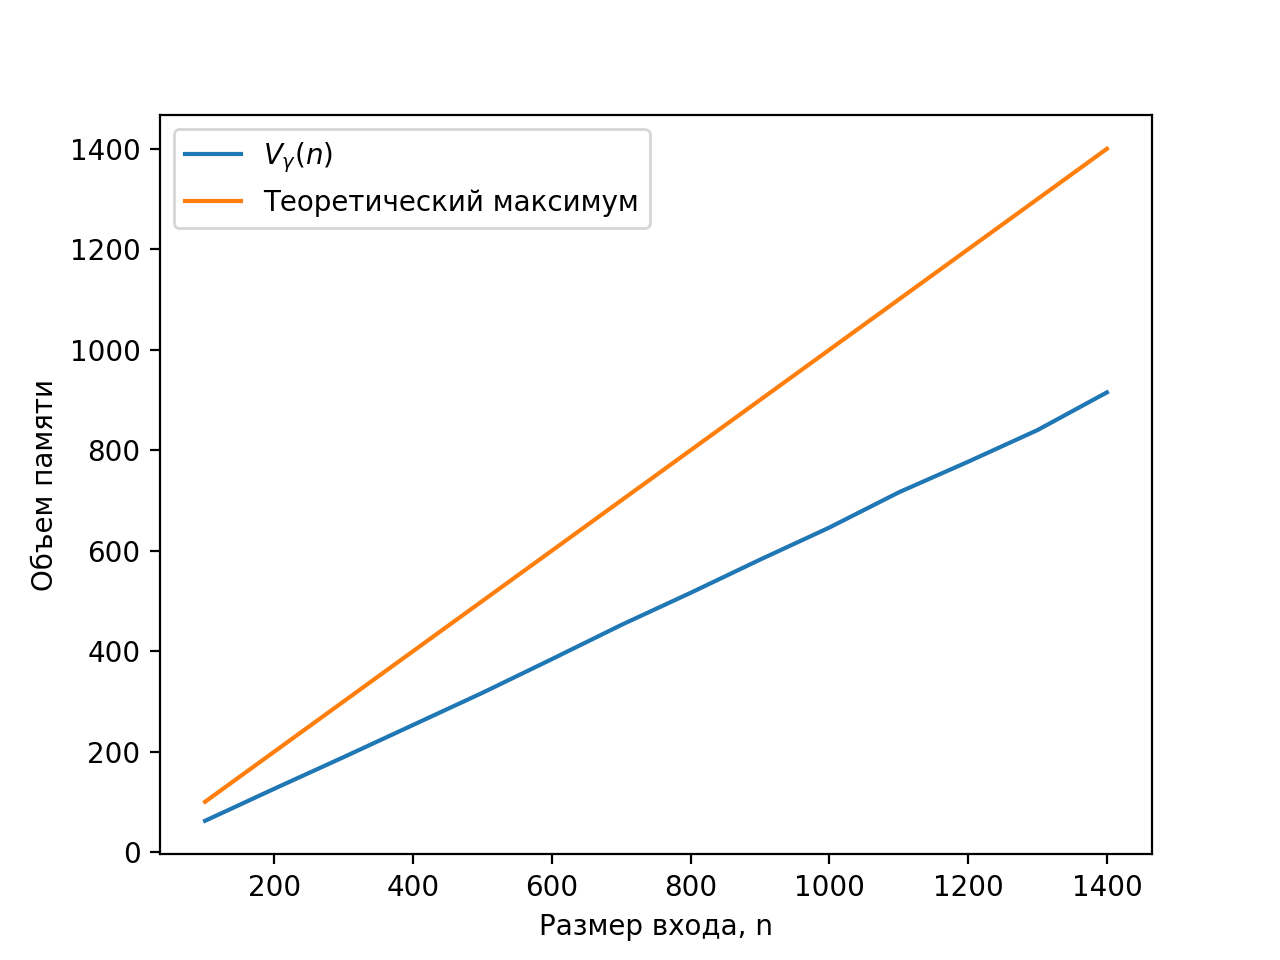
\includegraphics[width=0.7\linewidth]{images/general.png}}
\caption{График доверительной ресурсоемкости и ресурсоемкости в худшем случае для алгоритма Левита}
\label{ris:image1}
\end{figure}

\pagebreak
\section{Создание автоматизированной системы}

Система должна быть легкой и понятной в использовании, доступной, а также должна быть написана на общеизвестных языках программирования. Последний пункт необходим, для дальнейшей модернизацией системы со стороны исследователей и разработчиков.

Был разработан web-сайт --- такое решение не требует установки приложений на устройства. Сайт позволяет загружать данные работы алгоритма, после этого проводит анализ и выгружает результаты на страницу.

В качестве стека технологий для разработки сайта были выбраны:\\
• Бэкенд
\par
--- NGINX --- веб-сервер, работающий на Unix-подобных операционных системах. Был использован, так как имеет ряд преимуществ: малый размер, масштабируемость, простота конфигурации, активная поддержка сообщества, хорошую документацию.
\par
--- Flask --- микрофреймворк для создания веб-приложений написанный на языке программирования Python. Микрофреймворк по размеру является небольшим решением и служит как базовый инструментарий, не реализуя ничего лишнего. Тем не менее, этого достаточно для данной работы. Был использован для реализации основных функции API для сбора, обработки и анализа.

\noindent• Фронтенд
\par
--- JavaScript --- мультипарадигменный язык программирования, был создан для того, чтобы делать веб-страницы <<живыми>>. Программы написанные на этом языке именуются скриптами. Позволяют использоваться в HTML и выполняются при загрузке веб-страницы автоматически. Среди языков для разработки интерфейсов в браузере является распространённым решением.
\par
--- AJAX --- аббревиатура от Asynchronous JavaScript and XML. С помощью этой технологии представляется возможным обмен данными браузера с сервером в <<фоновом>> режиме. В результате такого принципа веб-страница не перезагружается полностью при обновлении данных. Таким образом, веб-приложения становятся быстрее и удобнее.

\begin{figure}[h!]
\center{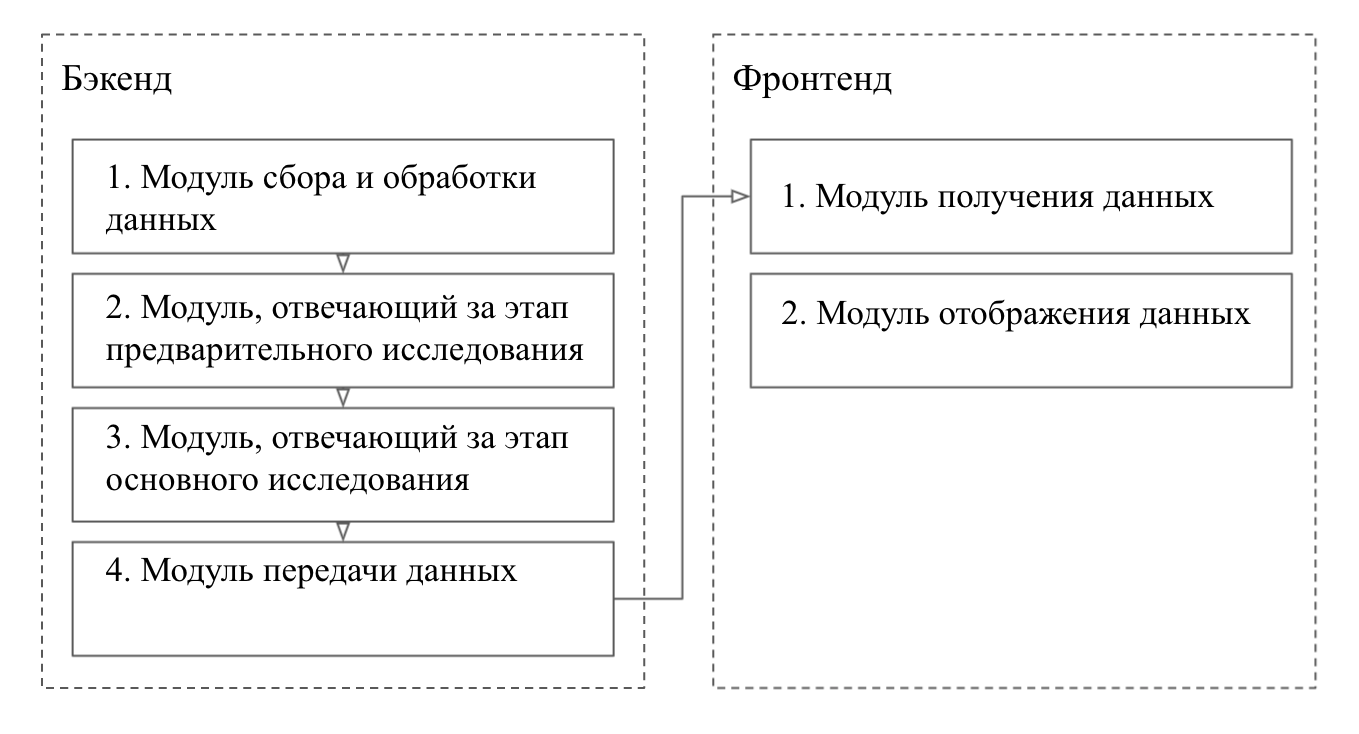
\includegraphics[width=1\linewidth]{images/architecture.png}}
\caption{Архитектура программной реализации}
\label{ris:image1}
\end{figure}

\pagebreak

\specialsection{Выводы}

Доверительная ресурсоемкость получена для значения коэффициента доверия $\gamma = 0.95$, т. е. в $95\%$ случаев наблюдаемая в единичном эксперименте ресурсоемкость алгоритма не будет превышать значение доверительной ресурсоемкости. Для рассматриваемого алгоритма эти значения меньше ресурсоемкости в худшем случае на исследуемом промежутке длин входа. Это означает, что с помощью апостериорного анализа можно лучше прогнозировать затраты памяти и более эффективно  выбирать оптимальный алгоритм, проводя сравнительный анализ функций доверительной ресурсоемкости.

Созданная автоматизированная система принимает на вход данные работы любого алгоритма и на них проводит анализ. После чего пользователю выводятся результаты анализа.

\pagebreak

\specialsection{Заключение}

В данной работе построена функция доверительной ресурсоемкости для алгоритма Левита. Также реализована автоматизированная система в виде сайта, через которую можно проводить анализ, загружая данные работы алгоритма.
\par
Исходный код всех программ находится в публичном репозитории в GitHub [16].

\pagebreak

% Библиография в cpsconf стиле
% Аргумент {1} ниже включает переопределенный стиль с выравниванием слева

\begin{thebibliography}{1}

\bibitem{voс1} Переписать базу сообщений с нуля и выжить [Электронный ресурс] // URL: url: https://vk.com/blog/messages-database (дата обращения: 20.01.2021)
\bibitem{voс2} Трахтенброт Б. А. Сложность алгоритмов и вычислений. Новосибирск: Изд-во Новосибирского ун-та, 1967.
\bibitem{voс3} Офман Ю. П. Об алгоритмической сложности дискретных функций // ДАН СССР. 1962. Т. 45, вып. 1. С. 48–51.
\bibitem{voс4} Маркова Н. А. Качество программы и его измерения // Системы и средства информатики. Вып. 12. — М.: Наука, 2002. С. 170–188.
\bibitem{voс5} Cormen T. H., Leiserson C. E., Rivest R. L., Stein C. Introduction to Algorithms. Chapter 1: Foundations (Second ed.) // Cambridge, MA: MIT Press and McGraw-Hill. 2001. P. 3–122.
\bibitem{voс6} Кнут Д. Э. Искусство программирования, том 1. Основные алгоритмы, 3-е изд.: Пер. с англ. — М.: Издательский дом «Вильямс», 2002. — 720 с.
\bibitem{voс7} Ахо А., Хопкрофт Дж., Ульман Дж. Построение и анализ вычислительных алгоритмов: Пер. с англ.: — М.: Мир, 1979. — 546 с.
\bibitem{voс8} Петрушин В. Н., Ульянов М. В., Кривенцов А. С. Доверительная трудоемкость — новая оценка качества алгоритмов // Информационные технологии и вычислительные системы. 2009. № 2. С. 23–37.
\bibitem{voс9} Петрушин В. Н., Ульянов М. В. Планирование экспериментального исследования трудоемкости алгоритмов на основе бета-распределения // Информационные технологии и вычислительные системы. 2008. № 2. С. 81–91.
\bibitem{voс10} Hutter F., Xu L. Hoos H., Leyton – Brown K. Algorithm runtime prediction: Methods & evaluation // Artificial Intelligence. 2014. Vol. 206. No 1. P. 79–111.
\bibitem{voс11} Erik D. Demaine, Jayson Lynch, Geronimo J. Mirano, Nirvan Tyagi. Energy-Efficient Algorithms. May 30, 2016
\bibitem{voс12} Петрушин В. Н., Ульянов М. В. Информационная чувствительность компьютерных алгоритмов. М.: Физматлит, 2010.
\bibitem{voс13} Ульянов М. В. Система обозначений в анализе ресурсной эффективности вычислительных алгоритмов // Вестн. МГАПИ. Сер. Естеств. и инж. науки. 2004. No1 (1). С. 42–49.
\bibitem{voс14} Pallottino S. Shortest-path methods: Complexity, interrelations and new propositions // Networks. 1984. Vol. 14. P. 257–267.
\bibitem{voс15} Королюк В. С., Портенко Н. И., Скороход А. В., Турбин А. Ф. Справочник по теории вероятностей и математической статистике. М.: Наука, 1985.
\bibitem{voс16} Репозиторий проекта в системе контроля версий GitHub [Электронный ресурс]: URL: https://github.com/romanychev-l/apostorial\_analysis (дата обращения: 31.05.2021)
\end{thebibliography}

\end{document}